%------------------------------------------------------------------------------------------------%

\chapter{Mesh Generation}

%------------------------------------------------------------------------------------------------%

%------------------------------------------------------------------------------------------------%
\section{How to use SPECFEM2D}
%------------------------------------------------------------------------------------------------%
The first step in running a spectral-element simulation consists of
constructing a high-quality mesh for the region under consideration.
We provide two possibilities to do so: (1) relying on an external,
hexahedral mesher, like Gmsh and CUBIT, or (2) using the provided, internal capabilities.
To run the mesher, please edit the main input file \texttt{DATA/Par\_file}, describing the setup of your simulation.
Then type:
%
\begin{verbatim}
    ./bin/xmeshfem2D
\end{verbatim}
%
to create the mesh, which will be stored in directory \texttt{OUTPUT\_FILES/}. \texttt{xmeshfem2D} will output several files called \texttt{Database??????.bin}, one for each process. These files are required for running the solver in a subsequent step.
%
\begin{figure}[htbp]
\centering
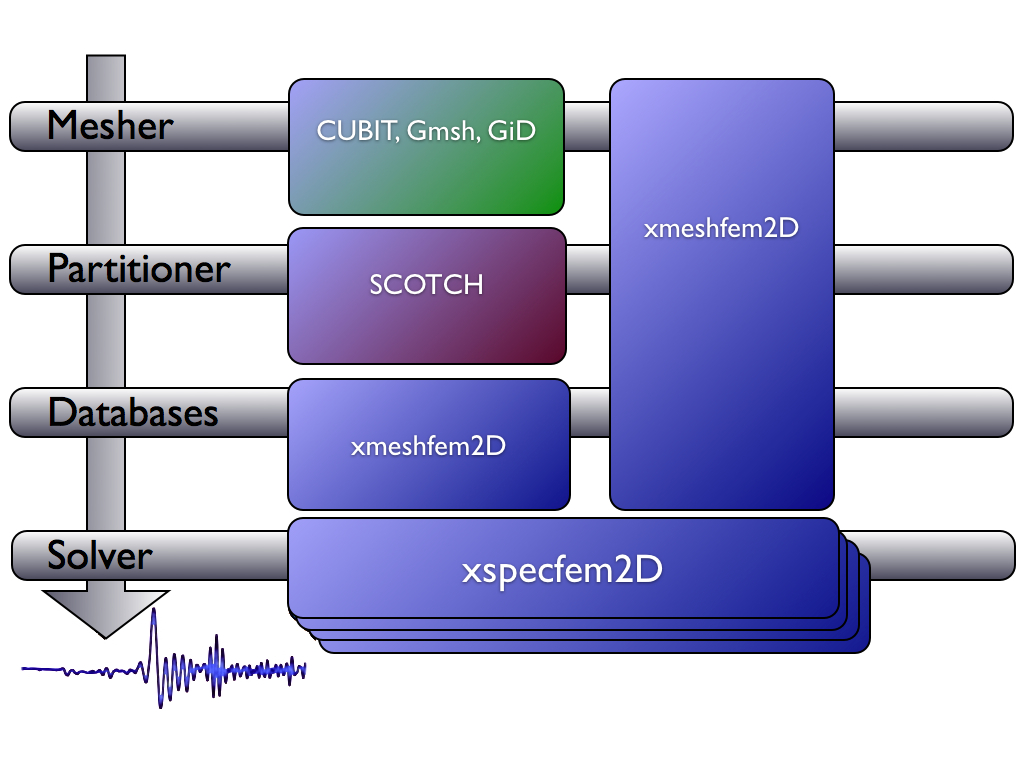
\includegraphics[width=.6\textwidth]{figures/workflow.pdf}

\caption{Schematic workflow for a SPECFEM2D simulation. The executable \texttt{xmeshfem2D} creates the GLL mesh points and assigns specific model parameters. The executable \texttt{xspecfem2D} solves the seismic wave propagation.}

\label{fig:workflow.databases}
\end{figure}


%------------------------------------------------------------------------------------------------%
\section*{Notes about \texttt{DATA/Par\_file} parameters}
%------------------------------------------------------------------------------------------------%

The default \texttt{DATA/Par\_file} provided in the root directory of the code contains detailed comments and should be almost self-explanatory
(note that some of the older \texttt{DATA/Par\_file} files provided in the \texttt{EXAMPLES} directory work fine but some of the comments
they contain may be obsolete or even wrong; thus refer to the default \texttt{DATA/Par\_file} instead for reliable explanations).\newline

If you need more details we do not have a detailed description of all the parameters for the 2D version in this manual
but you can find useful information in the manuals of the 3D versions, since many parameters and the general philosophy is similar. They are available at
\urlwithparentheses{https://github.com/SPECFEM/specfem3d/tree/master/doc/USER_MANUAL}.\newline

\begin{description}

\item[{\texttt{NPROC}}]
 If you have the code compiled with MPI support, you can specify the number of processes ($>1$) for the simulation to run on. Otherwise, this has to be set to 1 for a serial run. The mesher will use the partitioner specified by parameter \texttt{PARTITIONING\_TYPE} to load-balance the mesh for multiple processes.

\item[{\texttt{NGNOD}}]
 Regarding mesh point numbering in the files created by the mesher, we use the classical convention of 4-node and 9-node finite elements (\texttt{NGNOD = 4} or \texttt{NGNOD = 9}, respectively):
%
\begin{verbatim}
         4 . . . . 7 . . . . 3
         .                   .
         .         eta       .
         .         |         .
         8         9--xi     6
         .                   .
         .                   .
         .                   .
         1 . . . . 5 . . . . 2
\end{verbatim}
%
the local coordinate system being $\xi$ and $\eta$ (\texttt{xi} and \texttt{eta}).
Note that this convention is used to describe the geometry only. In the solver the wave field is then described based on high-order Lagrange interpolants
at Gauss-Lobatto-Legendre points, as is classical in spectral-element methods.


\item[{\texttt{MODEL}}]
 With \texttt{MODEL = default} chosen, a variety of simple velocity and density models can be defined using the \texttt{nbmodels} section in the \texttt{Par\_file}.

The material types can be specified by one of the following line formats:
%
\begin{verbatim}
I:  model_number 1 rho Vp Vs 0 0 QKappa Qmu 0 0 0 0 0 0
II:  model_number 2 rho c11 c13 c15 c33 c35 c55 c12 c23 c25 0 QKappa Qmu
III: model_number 3 rhos rhof phi c kxx kxz kzz Ks Kf Kfr etaf mufr Qmu
IV: model_number -1 0 0 A 0 0 0 0 0 0 0 0 0 0
\end{verbatim}
%
\begin{description}
\item[I:] To make a given region acoustic, use (I) and make \texttt{Vs} be zero. To make a given region isotropic elastic, use (I) and make \texttt{Vs} be nonzero.  See Section 4.1 for more details.

Thus, to create acoustic (fluid) regions, just set the S wave speed to zero and the code will see that these elements are fluid and switch to the right equations there automatically, and automatically match them with the solid regions.

\item[II:] To make a given region anisotropic, use (II).  See Section 4.3 for more details.

\item[III:] To make a given region poroelastic, use (III).  See Section 4.4 for more details.

\item[IV:] To impose a tomographic model on a given region, use (IV).  For now, we only allow for a single tomography file and region.
Note that the \texttt{model\_number} must be strictly positive, but the following domain number must be negative (-1) for tomographic models.
The values for density (rho) and Vp are ignored, however the value for Vs, i.e., \texttt{A}, must be either zero (0.0) to be recognized as an acoustic region or a positive non-zero value (e.g., 1.0) for an elastic region. The tomographic model values are overimposed on this region, and defined in the file specified by the parameter \texttt{TOMOGRAPHY\_FILE}.
\end{description}

When viscoelasticity is turned on, the \texttt{Vp} and \texttt{Vs} values that are read here are the UNRELAXED ones i.e. the values at infinite frequency
unless the \texttt{READ\_VELOCITIES\_AT\_f0} parameter is set to true, in which case they are the values at frequency $f_0$.
Please also note that Qmu is always equal to Qs, but Qkappa is in general not equal to Qp. To convert one to the other see \texttt{doc/note\_on\_Qkappa\_versus\_Qp.pdf} and \texttt{utils/attenuation/conversion\_from\_Qkappa\_Qmu\_to\_Qp\_Qs\_from\_Dahlen\_Tromp\_959\_960.f90}.

 With \texttt{MODEL = default} chosen, a variety of simple layered model configurations can be specified using the \texttt{nbregions} section in the \texttt{Par\_file}. Please see the comment in the \texttt{Par\_file} how to specify different material regions in the mesh for internal meshes. Meshes defined by an external mesher will have to specify these informations in separate files, please find more explanations below for the parameter \texttt{read\_external\_mesh}.

The parameter \texttt{MODEL} can also have other values specified than \texttt{default}. Possible selections are:
\begin{itemize}
\item \texttt{ascii}: for reading in a single ASCII model file (\texttt{DATA/proc***\_rho\_vp\_vs.dat})
\item \texttt{binary} or \texttt{gll}: for reading in binary model files (\texttt{DATA/proc***\_rho.bin}, \texttt{DATA/proc***\_vp.bin}, \texttt{DATA/proc***\_vs.bin}). In case attenuation is turned on for the simulation, it will also read in attenuation files (\texttt{DATA/proc***\_Qmu.bin}, \texttt{DATA/proc***\_Qkappa.bin}).
\item \texttt{binary\_voigt}: for reading in an anisotropic model specified by binary files (\texttt{DATA/proc***\_rho.bin}, \texttt{DATA/proc***\_c11.bin}, \texttt{DATA/proc***\_c13.bin}, \texttt{DATA/proc***\_c15.bin}, \texttt{DATA/proc***\_c33.bin}, \texttt{DATA/proc***\_c35.bin}, \texttt{DATA/proc***\_c55.bin})
\item \texttt{external}: for reading in a velocity model specified in the source code routine \texttt{define\_external\_model()} in file \texttt{src/specfem2d/define\_external\_model.f90}. The user can implement his own routine here as explained in the source file. By default, the routine implements the spherically symmetric isotropic AK135 model.
\item \texttt{legacy}: for reading in a single ASCII model file with a legacy format of very old SPECFEM2D versions (\texttt{DATA/proc***\_model\_velocity.dat\_input})
%\item \texttt{marmousi}: for imposing the Marmousi benchmark velocity model.
\end{itemize}


\item[{\texttt{read\_external\_mesh}}]
 If you are using an external mesher (like Gmsh, CUBIT/Trelis or GiD), you should set this parameter to \texttt{.true.}, with the following files defined for the mesher:
  \begin{description}
     \item[{\texttt{mesh\_file}}] is the file describing the mesh : first line is the number of elements, then a list of 4 nodes (quadrilaterals only) forming each elements on each line.

     \item[{\texttt{nodes\_coords\_file}}] is the file containing the coordinates ($x$ and $z$) of each node: number of nodes on the first line, then coordinates x and z on each line.

     \item[{\texttt{materials\_file}}] is the number of the material for every element : an integer ranging from 1 to \texttt{nbmodels} on each line.

     \item[{\texttt{free\_surface\_file}}] is the file describing the edges forming the acoustic free surface: number of edges on the first line, then on each line: number of the element, number of nodes forming the free surface (1 for a point, 2 for an edge), the nodes forming the free surface for this element. If you do not want any free surface, just put 0 on the first line; you then get a rigid surface instead.

     \item[{\texttt{axial\_elements\_file}}] is the file describing the axial elements in the case of an axisymmetric simulation. See Section~\ref{sec:axisym}.

     \item[{\texttt{absorbing\_surface\_file}}] is the file describing the edges forming the absorbing boundaries:
number of edges on the first line, then on each line: number of the element, number of nodes forming the absorbing edge (must always be equal to 2),
the two nodes forming the absorbing edge for this element, and then the type of absorbing edge: 1 for BOTTOM, 2 for RIGHT, 3 for TOP and 4 for LEFT.
Only two nodes per element can be listed, i.e., the second parameter of each line must always be equal to 2.
If one of your elements has more than one edge along a given absorbing contour
(e.g., if that contour has a corner) then list it twice,
putting the first edge on the first line and the second edge on the second line.
Do not list the same element with the same absorbing edge twice or more, otherwise absorption will not be correct because the edge integral
will be improperly subtracted several times.
If one of your elements has a single point along the absorbing contour rather than a full edge, do NOT list it
(it would have no weight in the contour integral anyway because it would consist of a single point).
If you use 9-node elements, list only the first and last points of the edge and not the intermediate point
located around the middle of the edge; the right 9-node curvature will be restored automatically by the code.

     \item[{\texttt{tangential\_detection\_curve\_file}}] contains points describing the envelope, that are used for the \texttt{source\_normal\_to\_surface} and \texttt{rec\_normal\_to\_surface}. Should be fine grained, and ordered clockwise. Number of points on the first line, then (x,z) coordinates on each line.
  \end{description}


\item[{\texttt{READ\_VELOCITIES\_AT\_f0}}]
 shift (i.e. change) velocities read from the input file to take average physical dispersion into account, i.e. if needed change the reference frequency at which these velocities are defined internally in the code: by default, the velocity values that are read at the end of this \texttt{Par\_file} of the code are supposed to be the unrelaxed values, i.e. the velocities at infinite frequency. If you set this flag to \texttt{.true.}, the values read are then those for a given frequency called \texttt{ATTENUATION\_f0\_REFERENCE}.

Note this only has an effect, if attenuation is turned on for the simulation, i.e., either \texttt{ATTENUATION\_VISCOELASTIC} or \texttt{ATTENUATION\_VISCOACOUSTIC} is set to \texttt{.true.}. Otherwise, the simulation is for a purely elastic or acoustic medium and the concept of a reference frequency is not needed.

\end{description}



%%
\begin{figure}[htbp]
\centering
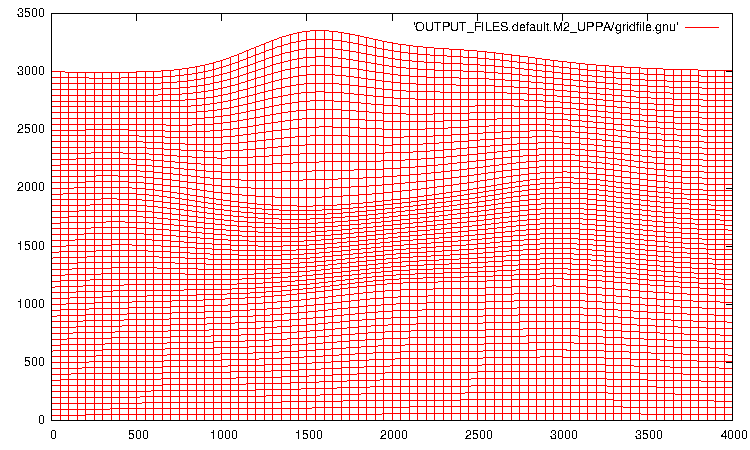
\includegraphics[width=3in]{figures/example-gridfile.pdf}
\caption{Example of a grid file generated by \texttt{xmeshfem2D} when parameter \texttt{output\_grid\_Gnuplot} is set to \texttt{.true.}, and visualized with gnuplot
(within gnuplot, type `\texttt{plot "OUTPUT\_FILES/gridfile.gnu" w l}').}
\label{fig:example.mesh}
\end{figure}


\section{How to use Gmsh to generate an external mesh}

Gmsh%
\footnote{freely available at the following address : \url{http://gmsh.info/}}
is a 3D finite element grid generator which can be used for the generation
of quadrangle and hexahedral meshes. It is therefore a good candidate
for generating meshes which can be processed by SPECFEM2D. Only two
modules of Gmsh are of interest for the SPECFEM2D users : the geometry
and the mesh modules. An example is given in directory \texttt{EXAMPLES/Gmsh\_example}
which illustrates the generation of an external mesh using these two
modules. The model that is considered consists of a homogeneous
square containing two circles filled with a different material.

The geometry is generated by loading file \texttt{SqrCirc.geo} into
Gmsh. The end of the \texttt{.geo} file contains several lines which
are required in order to define the sides of the box and the media.
This is done using the following conventions :
%
\begin{quote}
\texttt{\textit{Physical Line(\textquotedbl Top\textquotedbl)
= \{1\}; }}
\textsf{\textit{\small line corresponding to the top of the box}}

\texttt{\textit{Physical Line(\textquotedbl Left\textquotedbl)
= \{2\}; }}
\textsf{\textit{\small line corresponding to the left side of the box}}

\texttt{\textit{Physical Line(\textquotedbl Bottom\textquotedbl)
= \{3\}; }}
\textsf{\textit{\small line corresponding to the bottom of the box}}

\texttt{\textit{Physical Line(\textquotedbl Right\textquotedbl)
= \{4\}; }}
\textsf{\textit{\small line corresponding to the right side of the box}}

\texttt{\textit{Physical Surface(\textquotedbl M1\textquotedbl)
= \{10\}; }}
\textsf{\textit{\small surrounding medium}}

\texttt{\textit{Physical Surface(\textquotedbl M2\textquotedbl)
= \{11,12\}; }}
\textsf{\textit{\small interior of the two circles}}
\end{quote}
%
For instance, if you want to fill the two circles with two different
materials, you will have to write :
%
\begin{quote}
\texttt{\textit{Physical Surface(\textquotedbl M1\textquotedbl)
= \{10\}; }}
\textsf{\textit{\small surrounding medium}}

\texttt{\textit{Physical Surface(\textquotedbl M2\textquotedbl)
= \{11\}; }}
\textsf{\textit{\small interior of the big circle}}

\texttt{\textit{Physical Surface(\textquotedbl M3\textquotedbl)
= \{12\}; }}
\textsf{\textit{\small interior of the small circle}}
\end{quote}
%
and, consequently, you will have to define a new medium numbered \texttt{3}
in the \texttt{Par\_file}.

\begin{figure}[htbp]
\begin{centering}
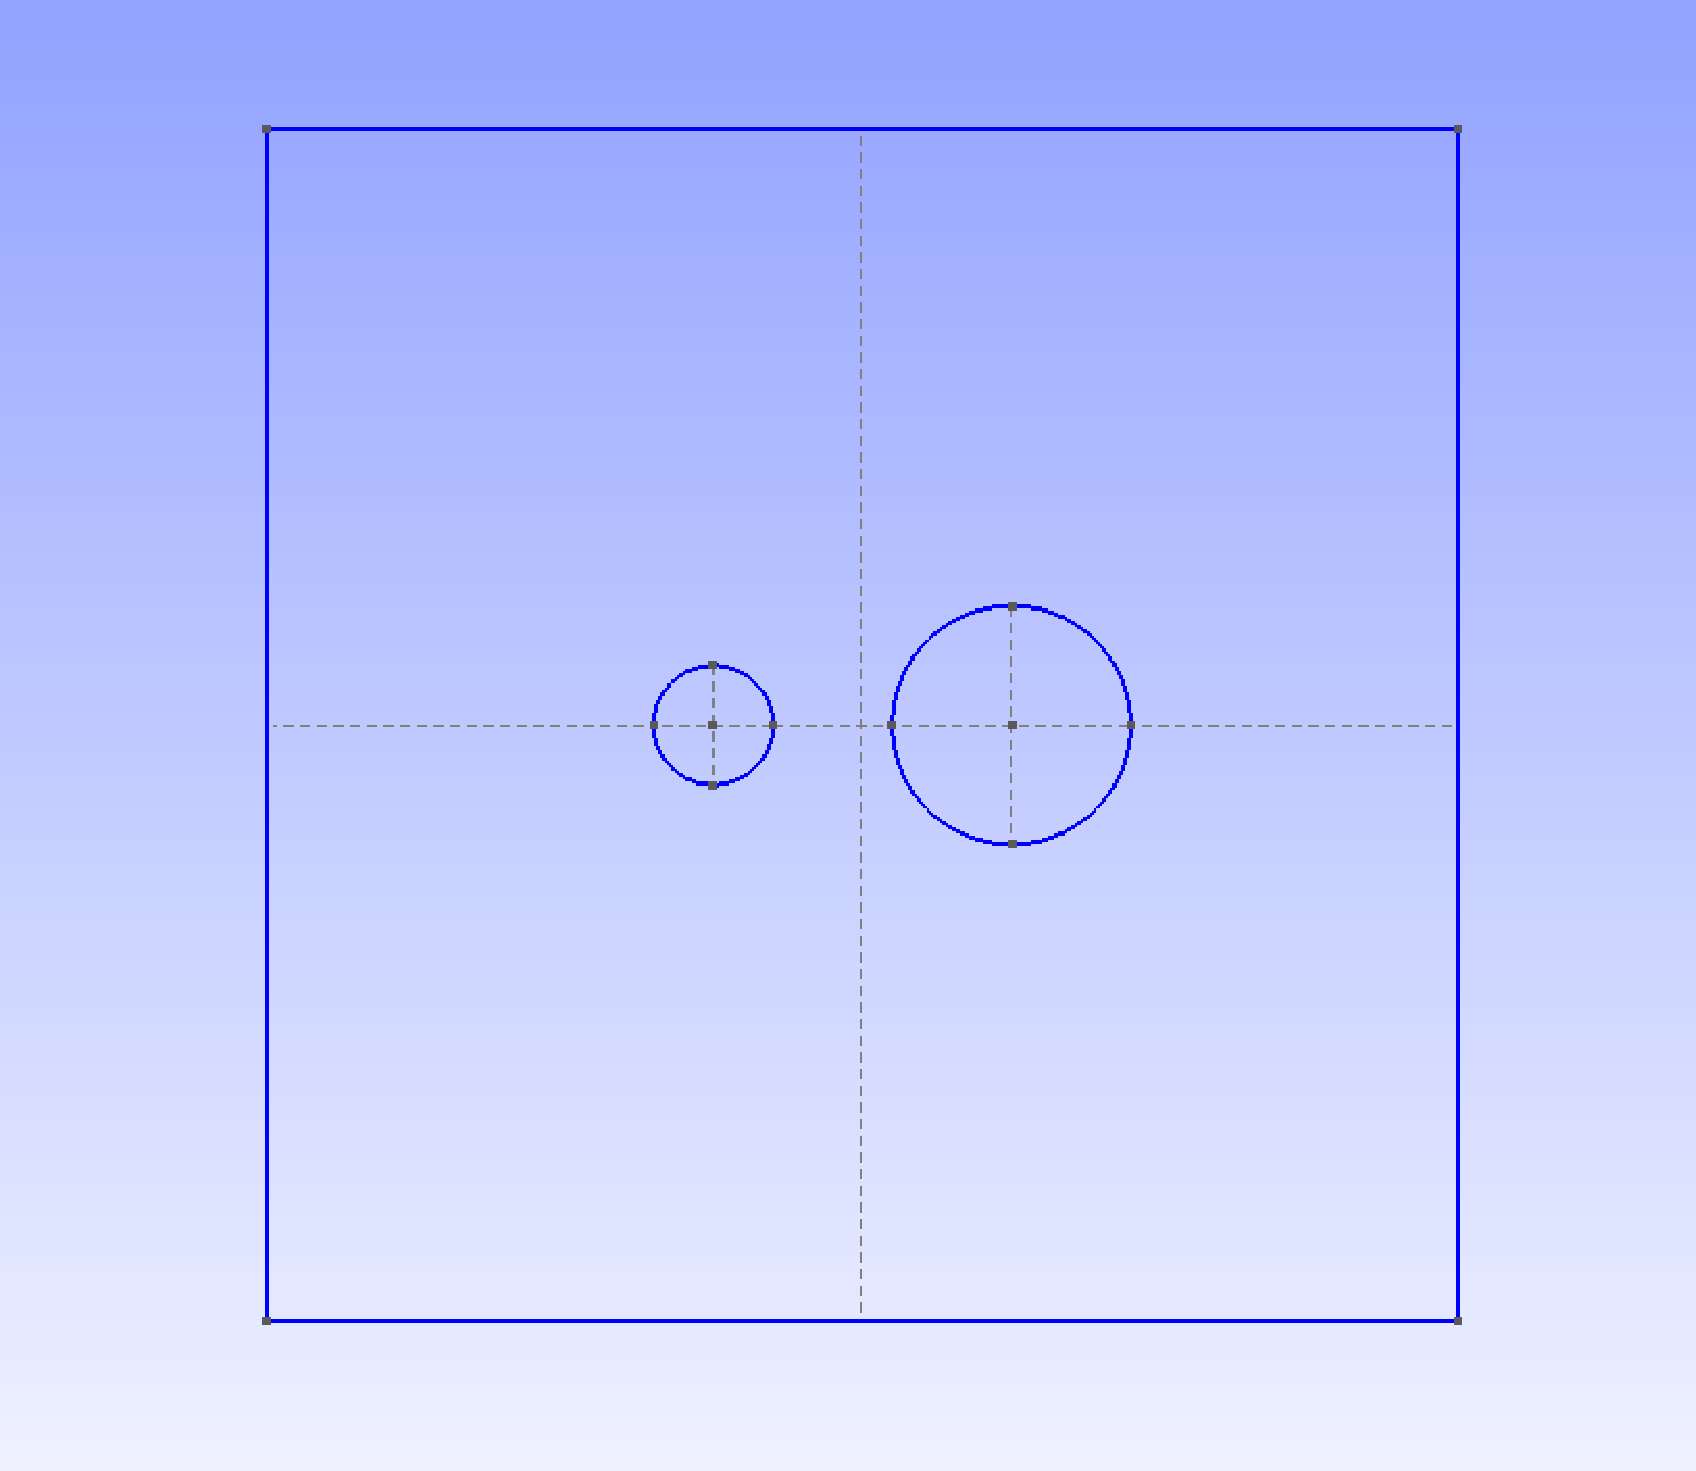
\includegraphics[width=0.481\columnwidth]{figures/Gmsh_geo.pdf}
\hspace{2mm}
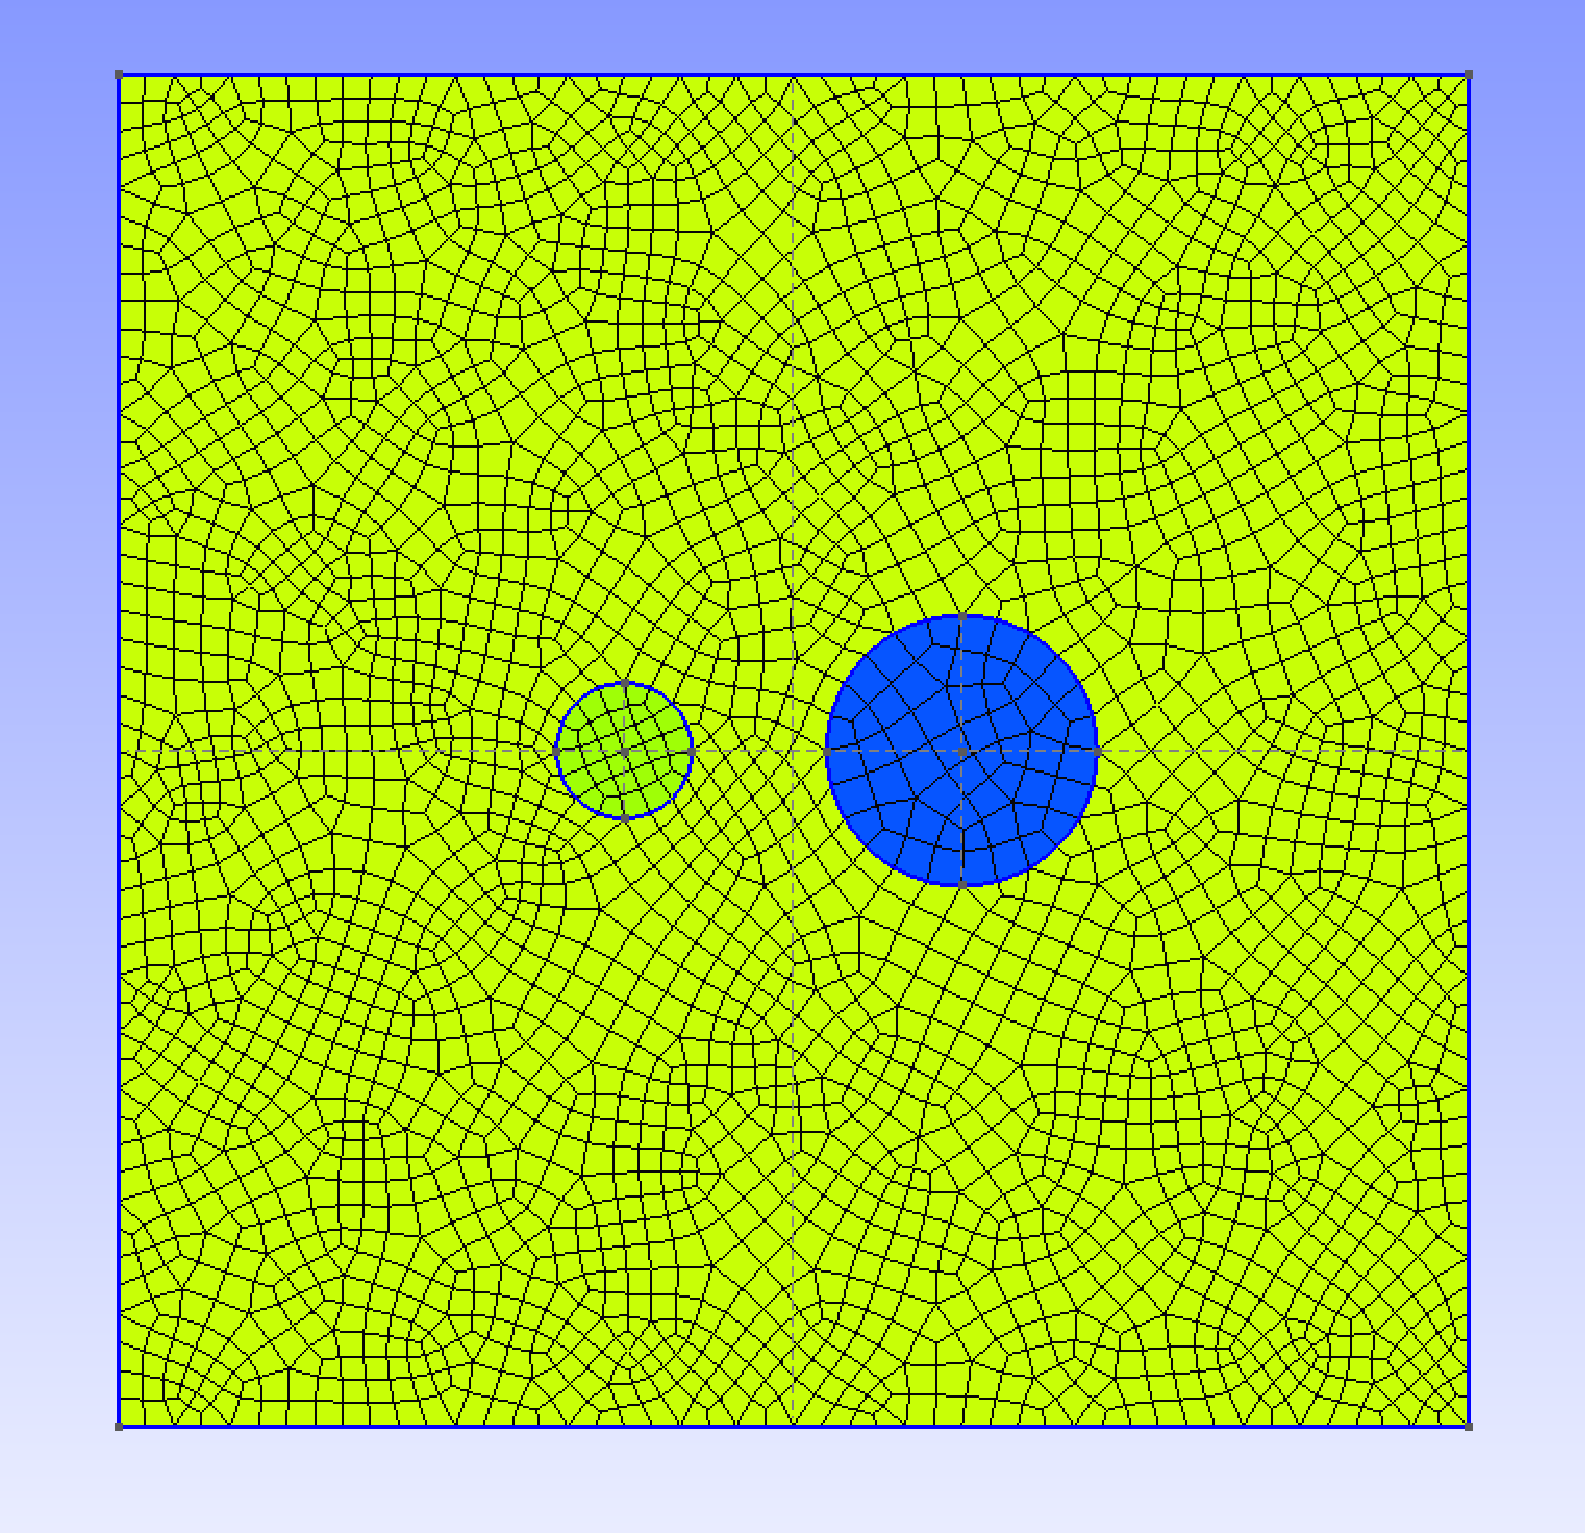
\includegraphics[width=0.43\columnwidth]{figures/Gmsh_Msh.pdf}
\end{centering}
\caption{Geometry and mesh of the two circle model generated with Gmsh}
\label{fig:Gmsh-example}
\end{figure}

Then, a 2D mesh can be created and saved after selecting the appropriate
options in Gmsh : \texttt{All quads} in \texttt{Subdivision algorithm}
and \texttt{1} or \texttt{2} in \texttt{Element order} whether you
want a 4 or 9 node mesh. This operation will generate a \texttt{SqrCirc.msh}
file which must be processed to get all the files required by SPECFEM2D
when using an external mesh (see previous section). This is done by
running a python script called \texttt{LibGmsh2Specfem.py}, located in
directory \texttt{utils/Gmsh}:
%
\begin{verbatim}
    python LibGmsh2Specfem.py SqrCirc -t A -b A -r A -l A
\end{verbatim}
%
Where the options \texttt{-t}, \texttt{-b},\texttt{ -r} and \texttt{-l}
represent the different sides of the model (top, bottom, right and
left) and can take the values \texttt{A} or \texttt{F} if the corresponding
side is respectively absorbing or free. All boundaries are absorbing
by default. The connections of the generated filenames to the filenames
indicated in the previous section are :
%
\begin{itemize}
\item \texttt{Mesh\_SqrCirc} is the \texttt{\textbf{mesh\_file}}
\item \texttt{Material\_SqrCirc} is the \texttt{\textbf{material\_file}}
\item \texttt{Nodes\_SqrCirc} is the\texttt{ }\texttt{\textbf{nodes\_coords\_file}}
\item \texttt{Surf\_abs\_SqrCirc} is the \texttt{\textbf{absorbing\_surface\_file}}
\item \texttt{Surf\_free\_SqrCirc} is the \texttt{\textbf{free\_surface\_file}}
\end{itemize}
%
In addition, four files like \texttt{free\_surface\_file} corresponding
to the sides of the model are generated.

\section{How to use Cubit/Trelis to generate an external mesh}
Trelis (that was known as Cubit)%
\footnote{available at \url{http://www.csimsoft.com/}}
is a 2D/3D finite element grid generator distributed by Csimsoft which can be
used for the generation of quadrangle and hexahedral meshes. Trelis has a convenient
interface with Python (module cubit) which allows to create meshes from Python scripts. To get
started with Cubit/Trelis we recommend you the step-by-step tutorials available at:
\url{http://www.csimsoft.com/tutorials.jsp}
Many powerful graphical tools are available, and very useful, but we will focus here on
the command line functionalities and especially the Python interface which is the real force of
Cubit/Trelis.

To get started we recommend to the inpatients to open Cubit/Trelis and to click on the
following symbol: \includegraphics[width=0.15in]{figures/play_journal_file.png}. Then select the
files of type Python Files (*.py) and play the following script:
\begin{verbatim}
    utils/cubit2specfem2d/simplest2DexampleWithPmls.py
\end{verbatim}
In the case you want to perform an axisymmetric simulation, we recommend you rather to play:
\begin{verbatim}
    utils/cubit2specfem2d/simpleAxisym2dMesh.py
\end{verbatim}
It will create a simple mesh with PMLs. Then re-click on \includegraphics[width=0.15in]{figures/play_journal_file.png} and
play:
\begin{verbatim}
    utils/cubit2specfem2d/cubit2specfem2d.py
\end{verbatim}
This script will create (in current directory) all the mesh files necessary for a SPECFEM2D simulation.
Other commented examples are available. We particularly recommend you to look at the folder \newline
\texttt{EXAMPLES/paper\_axisymmetry\_example}
beginning by reading the README available there.
Read carefully the comments in these scripts, they are helpful.
Another way to use Python together with Cubit/Trelis is to use the script tab.
This tab is a real Python terminal that can be used to pass command line python
instruction to Cubit/Trelis through the cubit module.
In the case of the Script tab is not visible in the command line panel (at the bottom of the screen) do:
\begin{verbatim}
    Tools -> Options... -> Layout [-> Cubit Layout] -> Show script tab
\end{verbatim}
This tab will allow you to play the scripts one line after another directly in Cubit/Trelis.
With this you should be able to understand how to create meshes and export them under SPECFEM2D format.

\subsection{Note about Cubit/Trelis built-in Python}
Beware, there are some (annoying) differences between cubit built-in Python and the actual Python langage:
\begin{itemize}
\item \texttt{"aString" + 'anotherString'} can cause problems even after being stored: \newline
      \texttt{a = "aString"} \newline
      \texttt{b = a + 'anotherString'} \newline
      Example which is not working:
\begin{verbatim}
pathToMeshDir = pathToSpecfem + 'EXAMPLES/paper_axisymmetry_example/MESH'
cubit.cmd('cd \"'+pathToMeshDir+'\"')
\end{verbatim}
\item No comments after double dots: \newline
      Example which is not working:
\begin{verbatim}
if True: # Just a dummy comment
    print "Ok!"
\end{verbatim}
      This example works without the comment.
\item \texttt{os.makedirs("\texttildelow/aDirectory/")} does not work. It creates a directory named \texttt{\texttildelow} \newline
       !!!!! To remove that do: \texttt{rm -R ./\texttildelow} AND NEVER \texttt{rm -rf \texttildelow} !!!!!
\item \texttt{sys.argv} can not be used
\item No comments \texttt{""" """} at the beginning of a script
\end{itemize}
And probably many others! Think about that before getting mad.

%------------------------------------------------------------------------------------------------%
\section{Notes about absorbing PMLs}
%------------------------------------------------------------------------------------------------%
If you use CPML, an additional file listing the CPML elements is needed.
Its first line is the total number of
CPML elements, and then a list of all the CPML elements, one per line.
The format of these lines is: in the first column the CPML element number, and in the second column a flag as follows:

\begin{table}[hb]
\caption{Definition of flags for CPML elements}
% title of Table
\centering
% used for centering table
\begin{tabular}{c l}
% centered columns (4 columns)
\hline\hline
%inserts double horizontal lines
Flag& Meaning\\ [0.5ex]
% inserts table
%heading
\hline
% inserts single horizontal line
1 & element belongs to a X CPML layer only (either in Xmin or in Xmax)\\
2 & element belongs to a Y CPML layer only (either in Ymin or in Ymax)\\
3 & element belongs to both a X and a Y CPML layer (i.e., to a CPML corner)\\ [1ex]
% [1ex] adds vertical space
\hline
%inserts single line
\end{tabular}
\label{table:CPMLflags}
% is used to refer this table in the text
\end{table}

In order to see how to add PML layers to a mesh / model created with an external mesher such as Gmsh, see the examples in directory
\texttt{EXAMPLES/CPML\_absorbing\_layers}.

If you use PML, the mesh elements that belong to the PML layers can be acoustic or elastic, but not viscoelastic nor poroelastic.
Then, when defining your model, you should define these absorbing elements as either acoustic or elastic.
If you forget to do that, the code will fix the problem by automatically converting the viscoelastic or poroelastic PML
elements to elastic. This means that strictly speaking the PML layer will not be perfectly matched any more, since the physical
model will change from viscoelastic or poroelastic to elastic at the entrance of the PML, but in practice this is sufficient and
produces only tiny / negligible spurious reflections.\newline

If you use PML and an external mesh (created using an external meshing tool
such as Gmsh, CUBIT/TRELIS or similar), try to have elements inside the PML as regular as possible,
i.e. ideally non-deformed rectangles obtained by `extrusion' of the edge mesh elements meshing the
outer edges of the computational domain without PML; by doing so, the PMLs obtained will be far more stable
in time (PML being weakly unstable from a mathematical point of view, very deformed mesh elements
inside the PMLs can trigger instabilities much more quickly).

If you have an existing CUBIT (or similar) mesh stored in SPECFEM2D
format but do not know how to assign CPML flags to it,
we have created a small serial Fortran program that will do that automatically for you.
That program is \texttt{utils/CPML/convert\_external\_layers\_of\_a\_given\_mesh\_to\_CPML\_layers2D.f90}.
When you create the PML layers using that script, you do not need to mark
(i.e. assign to physical entities with a specific name) those external layers in the mesher.
However you still need to specify the boundary of the mesh as you where doing in the case of absorbing conditions.
The script will automatically extract the elements on the PML. It will ask you for a thickness for the PML layers.
Suppose that you have created a region with a 1-meter size element, when it will prompt for the PML thickness
you can enter 3.1 and it will create a PML 3 element thick. Always input a slightly larger (5-10\%) size because the element might be slightly skewed,
or if you have not created your PML region via extrusion/webcut in CUBIT/TRELIS.\newline

To stabilize PMLs it also helps to add a transition layer of geometrically-regular non-PML elements, in which attenuation is also
turned off (i.e. $Q_\kappa = Q_\mu = 9999$ in that layer), as in the red layer of Figure~\ref{fig:mesh_extrusion}.
Our tools in directory in directory \texttt{utils/CPML} will implement that transition layer automatically in future.\newline

\noindent
To be more precise:
\begin{itemize}
\item [1/] If one wants to use PML layers, they should NOT mark the layers according to that python script - the reason is that the \texttt{xmeshfem2d} does not recognize those CPML flags. If whoever developed the script adjusts it to solve this problem - this might be a great relief for users; as of now no physical identifiers are needed for those layers.

\item [2/] HOWEVER, the "Top", "Bottom", "Left"," and "Right" boundaries of the model, need to be re-assigned to outer boundaries of the model - that will be the leftmost boundary of the left -bounding PML , rightmost of the right PML, topmost for the Top PML (if there is one) and the bottom boundary of the bottom layer. Those and only those lines need to have the mentioned identifiers (opposite to the example with the two-holed square with Stacey conditions).

\item [3/] There is no need to create Top PML in case one wants it to be reflective; as the fortran script that assigns the flag will ignore the elements that sit within  PML-layer thickness distance to the top.

\item [4/] The Fortran program \texttt{utils/CPML/convert\_external\_layers\_of\_a\_given\_mesh\_to\_CPML\_layers2D.f90}
that flags the PML elements does not create additional elements; it simply takes the elements within chosen distance from the boundaries, that sit in the interior of model and marks them as absorbing.
\end{itemize}

\noindent
If you use PML and an external velocity and density model (e.g., setting flag \texttt{MODEL} to \texttt{external}),
you should be careful because mathematically a PML cannot handle heterogeneities along the
normal to the PML edge inside the PML layer. This comes from the fact that the damping profile
that is defined assumes a constant velocity and density model along the normal
direction.
Thus, you need to modify your velocity and density model in order for it to be 1D inside
the PML, as shown in Figure~\ref{fig:modify_external_velocity_model_to_use_PML}.
This applies to the bottom layer as well; there you should make sure
that your model is 1D and thus constant along the vertical direction.\newline

To summarize, only use a 2D velocity and density model inside the physical region, and in
all the PML layers extend it by continuity from its values along the
inner PML edge.

%%
\begin{figure}[htbp]
\noindent \begin{centering}
\includegraphics[width=4.5in]{figures/how_to_use_a_transition_mesh_layer_to_stabilize_PML.png}
\par\end{centering}
\caption{Mesh extrusion for PML (green elements) and a non-PML stabilization layer (red elements).}
\label{fig:mesh_extrusion}
\end{figure}
%%

%%
\begin{figure}[htbp]
\centering
\includegraphics[width=6in]{figures/how_to_use_PML_with_external_velocity_model.pdf}
\caption{How to modify your external 2D velocity and density model in order to use PML.
Such a modification is not needed when using Stacey absorbing boundary conditions (but such conditions
are significantly less efficient).}
\label{fig:modify_external_velocity_model_to_use_PML}
\end{figure}
%%

%------------------------------------------------------------------------------------------------%
\section{Controlling the quality of an external mesh}
%------------------------------------------------------------------------------------------------%

To examine the quality of the elements in your externally build mesh, type
%
\begin{verbatim}
    ./bin/xcheck_quality_external_mesh
\end{verbatim}
%
(and answer "3" to the first question asked).
This code will tell you which element in the whole mesh has the worst quality (maximum skewness, i.e. maximum deformation of the element angles) and it should be enough to modify this element with the external software package used for the meshing, and
to repeat the operation until the maximum skewness of the whole mesh is less or equal to about 0.75 (above is dangerous: from 0.75 to 0.80 could still work, but if there is a single element above 0.80 the mesh should be improved).

The code also shows a histogram of 20 classes of skewness which tells how many element are above the skewness = 0.75, and to which percentage of the total this amounts. To see this histogram, you could type:
%
\begin{verbatim}
    gnuplot plot_mesh_quality_histogram.gnu
\end{verbatim}
%
This tool is useful to estimate the mesh quality and to see it evolve along the successive corrections.

%------------------------------------------------------------------------------------------------%
\section{Controlling how the mesh samples the wave field}
%------------------------------------------------------------------------------------------------%

To examine (using Gnuplot) how the mesh samples the wave field, type
%
\begin{verbatim}
    gnuplot plot_points_per_wavelength_histogram.gnu
\end{verbatim}
%
and also check the following histogram printed on the screen or in the output file:
%
\begin{verbatim}
    histogram of min number of points per S wavelength (P wavelength in
    acoustic regions)
    (too small: poor resolution of calculations - too big = wasting
    memory and CPU time)
    (threshold value is around 4.5 points per wavelength in elastic media
    and 5.5 in acoustic media)
\end{verbatim}

If you see that you have a significant number of mesh elements below the threshold indicated, then your simulations
will not be accurate and you should create a denser mesh. Conversely, if you have a significant number of mesh elements above the threshold indicated,
the mesh your created is too dense, it will be extremely accurate but the simulations will be slow; using a coarser mesh would be sufficient and would lead to faster simulations.


